% Final-presentation slide deck for CS5330 final project:
% "A From-Scratch CUDA Forward-Pass Inference Engine for a LeNet-Style
%  MNIST CNN."
%
% Target: a ~12-13 minute recorded talk (slot: <=15 min). Reuses the
% figures under ../report/figs/ and the fusion-memory-traffic TikZ
% from the IEEE report so the visual language is consistent with the
% submitted paper.
%
% Build: pdflatex slides.tex (twice for references). Requires the
% `metropolis` Beamer theme; the IfFileExists guard falls back cleanly
% to the default theme if it isn't installed.

\documentclass[aspectratio=169,10pt]{beamer}

% --- Theme ---------------------------------------------------------------
\IfFileExists{beamerthememetropolis.sty}{%
  \usetheme{metropolis}
  \metroset{progressbar=frametitle, numbering=fraction, block=fill}
}{%
  \usetheme{default}
  \usecolortheme{seahorse}
  \setbeamertemplate{navigation symbols}{}
}

\usepackage{graphicx}
\usepackage{booktabs}
\usepackage{tikz}
\usetikzlibrary{positioning,arrows.meta,calc,fit}
\usepackage{xcolor}
\usepackage{colortbl}
\usepackage{amsmath}
\usepackage{listings}
\usepackage{pifont}  % for \ding{51} checkmark
\newcommand{\chk}{\textcolor{green!55!black}{\ding{51}}\,}

\graphicspath{{../report/figs/}}

% --- Northeastern University palette -------------------------------------
\definecolor{NURed}{HTML}{CC0000}
\definecolor{NURedDark}{HTML}{990000}
\definecolor{NURedLight}{HTML}{FFEAEA}
\definecolor{NUGray}{HTML}{4E4E4E}
\definecolor{NULightGray}{HTML}{D6D6D6}

% Override metropolis accent (progress bar, alerted text) to NU Red
\setbeamercolor{progress bar}{fg=NURed, bg=NURed!25}
\setbeamercolor{alerted text}{fg=NURed}
\setbeamercolor{frametitle}{bg=NUGray}

% --- CUDA listing style --------------------------------------------------
\definecolor{lstbg}{RGB}{250,248,246}
\definecolor{lstkw}{RGB}{153,0,0}
\definecolor{lstcm}{RGB}{110,110,110}
\definecolor{lststr}{RGB}{120,60,40}
\lstdefinelanguage{CUDA}[]{C++}{%
  morekeywords={__global__,__device__,__host__,__shared__,__restrict__,
                __syncthreads,extern,fmaxf,blockIdx,threadIdx,blockDim,
                gridDim,cudaMemcpy,cudaMalloc,cudaFree},
}
\lstset{
  language=CUDA,
  basicstyle=\ttfamily\scriptsize,
  keywordstyle=\color{lstkw}\bfseries,
  commentstyle=\color{lstcm}\itshape,
  stringstyle=\color{lststr},
  backgroundcolor=\color{lstbg},
  frame=single,
  rulecolor=\color{black!20},
  framesep=3pt,
  xleftmargin=6pt,
  xrightmargin=2pt,
  showstringspaces=false,
  breaklines=true,
  columns=fullflexible,
  escapeinside={(*}{*)},
}

% --- Title-block metadata -----------------------------------------------
\title{A From-Scratch CUDA CNN}
\subtitle{Forward-pass inference for LeNet-MNIST, no framework at runtime}
\author{Ashish Dasu}
\institute{CS5330 Pattern Recognition and Computer Vision\\[2pt]
           Khoury College of Computer Sciences, Northeastern University\\[2pt]
           Prof.\ Bruce Maxwell}
\date{April 2026}

\begin{document}

% ── Slide 1 ─ Title ──────────────────────────────────────────────────────────
\begin{frame}[plain]
  \titlepage
\end{frame}

% ── Slide 2 ─ Pipeline + Correctness ─────────────────────────────────────────
\begin{frame}{The network and how we verified it}
  \centering
  \resizebox{0.96\linewidth}{!}{%
  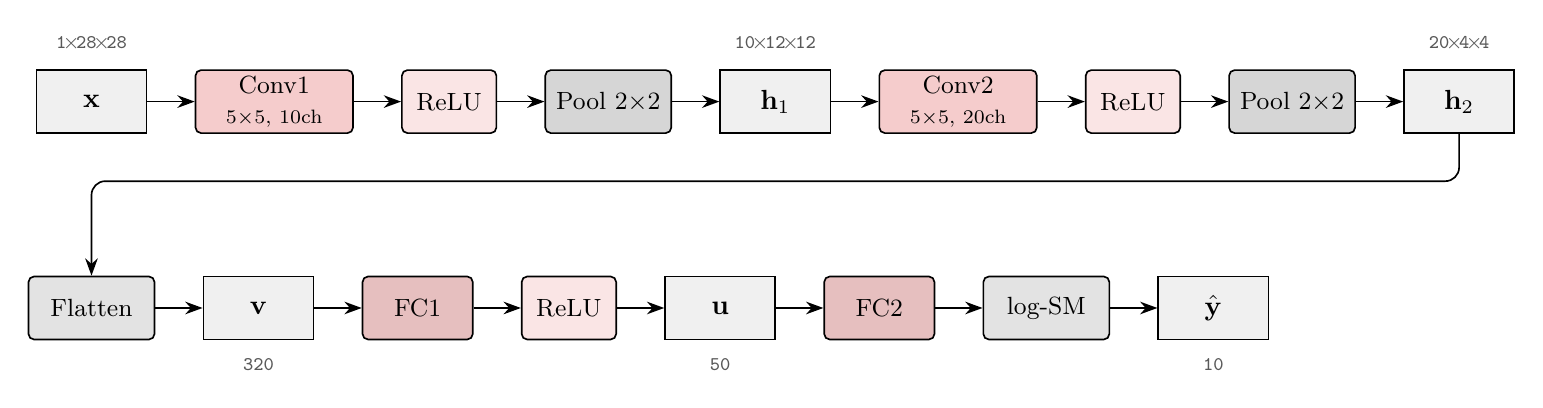
\begin{tikzpicture}[
    tnode/.style={draw, semithick, fill=gray!12, minimum height=8mm,
                  minimum width=14mm, align=center, inner sep=2pt,
                  font=\normalsize\bfseries},
    conv/.style={draw, semithick, rounded corners=2pt, fill=NURed!20,
                 minimum height=8mm, minimum width=20mm,
                 align=center, inner sep=2pt, font=\small},
    pool/.style={draw, semithick, rounded corners=2pt, fill=NULightGray,
                 minimum height=8mm, minimum width=16mm,
                 align=center, inner sep=2pt, font=\small},
    relu/.style={draw, semithick, rounded corners=2pt, fill=NURed!10,
                 minimum height=8mm, minimum width=12mm,
                 align=center, inner sep=2pt, font=\small},
    fcop/.style={draw, semithick, rounded corners=2pt, fill=NURedDark!25,
                 minimum height=8mm, minimum width=14mm,
                 align=center, inner sep=2pt, font=\small},
    misc/.style={draw, semithick, rounded corners=2pt, fill=gray!22,
                 minimum height=8mm, minimum width=16mm,
                 align=center, inner sep=2pt, font=\small},
    shp/.style={font=\scriptsize\ttfamily, text=black!65},
    ar/.style={-{Stealth[length=2.2mm,width=1.6mm]}, semithick},
    node distance=6mm,
  ]
    % ── Row 1: x → conv stage 1 → h1 → conv stage 2 → h2 ──────────────
    \node[tnode] (x) {$\mathbf{x}$};
    \node[shp, above=3pt of x] {1$\!\times\!$28$\!\times\!$28};

    \node[conv, right=of x]  (c1) {Conv1\\{\scriptsize 5$\times$5, 10ch}};
    \node[relu, right=of c1] (r1) {ReLU};
    \node[pool, right=of r1] (p1) {Pool 2$\times$2};
    \node[tnode, right=of p1] (h1) {$\mathbf{h}_1$};
    \node[shp, above=3pt of h1] {10$\!\times\!$12$\!\times\!$12};

    \node[conv, right=of h1]  (c2) {Conv2\\{\scriptsize 5$\times$5, 20ch}};
    \node[relu, right=of c2]  (r2) {ReLU};
    \node[pool, right=of r2]  (p2) {Pool 2$\times$2};
    \node[tnode, right=of p2] (h2) {$\mathbf{h}_2$};
    \node[shp, above=3pt of h2] {20$\!\times\!$4$\!\times\!$4};

    % ── Row 2: flatten → FC stage 1 → u → FC stage 2 → ŷ ───────────────
    \node[misc, below=18mm of x] (fl) {Flatten};
    \node[tnode, right=of fl]    (v)  {$\mathbf{v}$};
    \node[shp, below=3pt of v]   {} ;
    \node[shp, below=3pt of v]   {320};
    \node[fcop, right=of v]      (fc1){FC1};
    \node[relu, right=of fc1]    (r3) {ReLU};
    \node[tnode, right=of r3]    (u)  {$\mathbf{u}$};
    \node[shp, below=3pt of u]   {50};
    \node[fcop, right=of u]      (fc2){FC2};
    \node[misc, right=of fc2]    (sm) {log-SM};
    \node[tnode, right=of sm]    (y)  {$\hat{\mathbf{y}}$};
    \node[shp, below=3pt of y]   {10};

    % ── Arrows row 1 ─────────────────────────────────────────────────────
    \foreach \a/\b in {x/c1, c1/r1, r1/p1, p1/h1,
                       h1/c2, c2/r2, r2/p2, p2/h2}
      \draw[ar] (\a) -- (\b);

    % ── Step-down: h2 → Flatten ──────────────────────────────────────────
    \draw[ar, rounded corners=5pt]
      (h2.south) -- ++(0,-6mm) -| (fl.north);

    % ── Arrows row 2 ─────────────────────────────────────────────────────
    \foreach \a/\b in {fl/v, v/fc1, fc1/r3, r3/u,
                       u/fc2, fc2/sm, sm/y}
      \draw[ar] (\a) -- (\b);
  \end{tikzpicture}}

  \vspace{0.4em}
  \footnotesize
  \textbf{Correctness:} CPU ref $\to$ per-kernel diff ($10^{-4}$ tol) $\to$
  10k MNIST end-to-end. \quad
  Max err \textbf{$1.91\!\times\!10^{-5}$} $\cdot$
  argmax \textbf{100\%} match $\cdot$
  accuracy \textbf{97.93\%}.
\end{frame}

% ── Slide 3 ─ CUDA Primer ────────────────────────────────────────────────────
\begin{frame}{Background: a CUDA kernel, in one slide}
  \begin{columns}[T,onlytextwidth]
  \begin{column}{0.48\textwidth}
    \textbf{Parallelism model.} A kernel launch is one program
    executed by many threads at once.
    \vspace{0.3em}
    \begin{center}
    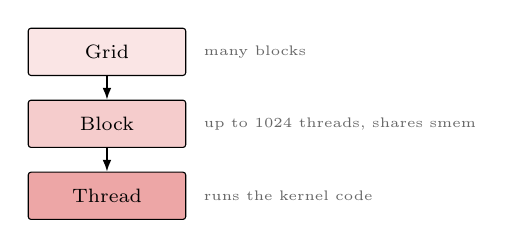
\begin{tikzpicture}[scale=0.75,
        lvl/.style={draw, rounded corners=1pt, minimum height=6mm,
                    minimum width=20mm, font=\scriptsize, inner sep=2pt,
                    align=center},
        ar/.style={-{Latex[length=1.5mm]}, semithick},
        note/.style={font=\tiny, text=black!60},
      ]
      \node[lvl, fill=NURed!10] (grid) {Grid};
      \node[lvl, fill=NURed!20, below=3mm of grid] (blk) {Block};
      \node[lvl, fill=NURed!35, below=3mm of blk] (thr) {Thread};
      \draw[ar] (grid) -- (blk);
      \draw[ar] (blk) -- (thr);
      \node[note, right=1mm of grid] {many blocks};
      \node[note, right=1mm of blk]  {up to 1024 threads, shares smem};
      \node[note, right=1mm of thr]  {runs the kernel code};
    \end{tikzpicture}
    \end{center}
    \vspace{0.2em}
    \scriptsize
    Threads in the same block can cooperate via
    \texttt{\_\_shared\_\_} memory and \texttt{\_\_syncthreads()};
    threads across blocks cannot.
  \end{column}
  \begin{column}{0.52\textwidth}
    \textbf{Memory hierarchy.} Latency costs dominate kernel design.
    \vspace{0.5em}
    \begin{center}
    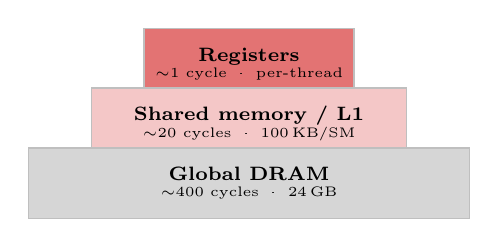
\begin{tikzpicture}[scale=0.88,
        mem/.style={draw=black!25, semithick, minimum height=9mm,
                    align=center, inner sep=4pt, font=\scriptsize},
      ]
      \node[mem, fill=NURed!55, minimum width=24mm] at (0,1.72)
            {\textbf{Registers}\\[-2pt]{\tiny $\sim$1 cycle \;·\; per-thread}};
      \node[mem, fill=NURed!22, minimum width=40mm] at (0,0.86)
            {\textbf{Shared memory / L1}\\[-2pt]{\tiny $\sim$20 cycles \;·\; 100\,KB/SM}};
      \node[mem, fill=NULightGray,  minimum width=56mm] at (0,0)
            {\textbf{Global DRAM}\\[-2pt]{\tiny $\sim$400 cycles \;·\; 24\,GB}};
    \end{tikzpicture}
    \end{center}
    \vspace{0.3em}
    \scriptsize
    \textbf{The whole talk is one idea:} move data from slow DRAM
    into fast shared memory / registers, reuse it, write results back.
  \end{column}
  \end{columns}
\end{frame}

% ── Slide 4 ─ Tiled Conv ─────────────────────────────────────────────────────
\begin{frame}{Opt.\ 1 --- tiled shared-memory convolution}
  \begin{columns}[c,onlytextwidth]
  \begin{column}{0.42\textwidth}
    \small One block $\to$ one 16$\times$16 output tile. Threads
    cooperatively load input + halo into \texttt{\_\_shared\_\_}
    memory per channel; read shmem instead of DRAM.

    \begin{center}
    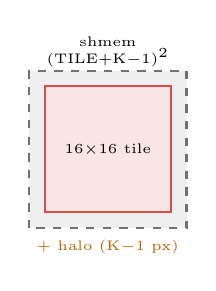
\begin{tikzpicture}[scale=0.40,
        inner/.style={draw=NURed!70, thick, fill=NURed!10},
        halo/.style={draw=NUGray!80, thick, dashed, fill=NULightGray!40},
        lab/.style={font=\tiny},
      ]
      \fill[halo] (-0.5,-0.5) rectangle (4.5,4.5);
      \fill[inner] (0,0) rectangle (4,4);
      \draw[halo] (-0.5,-0.5) rectangle (4.5,4.5);
      \draw[inner] (0,0) rectangle (4,4);
      \node[lab] at (2,2) {16$\times$16 tile};
      \node[lab, text=orange!75!black] at (2,-1.1) {+ halo (K$-$1 px)};
      \node[lab, align=center] at (2,5.1) {shmem\\(TILE+K$-$1)$^2$};
    \end{tikzpicture}
    \end{center}

    \scriptsize Reuse factor $=K_h{\cdot}K_w=25$. At LeNet scale the
    working set already fits in L1 --- \textbf{naive wins.} Same tile
    strategy wins \textbf{6.4$\times$} on a large GEMM (next slide).
    The \emph{regime} decides.
  \end{column}
  \begin{column}{0.58\textwidth}
    \vfill
    \centering
    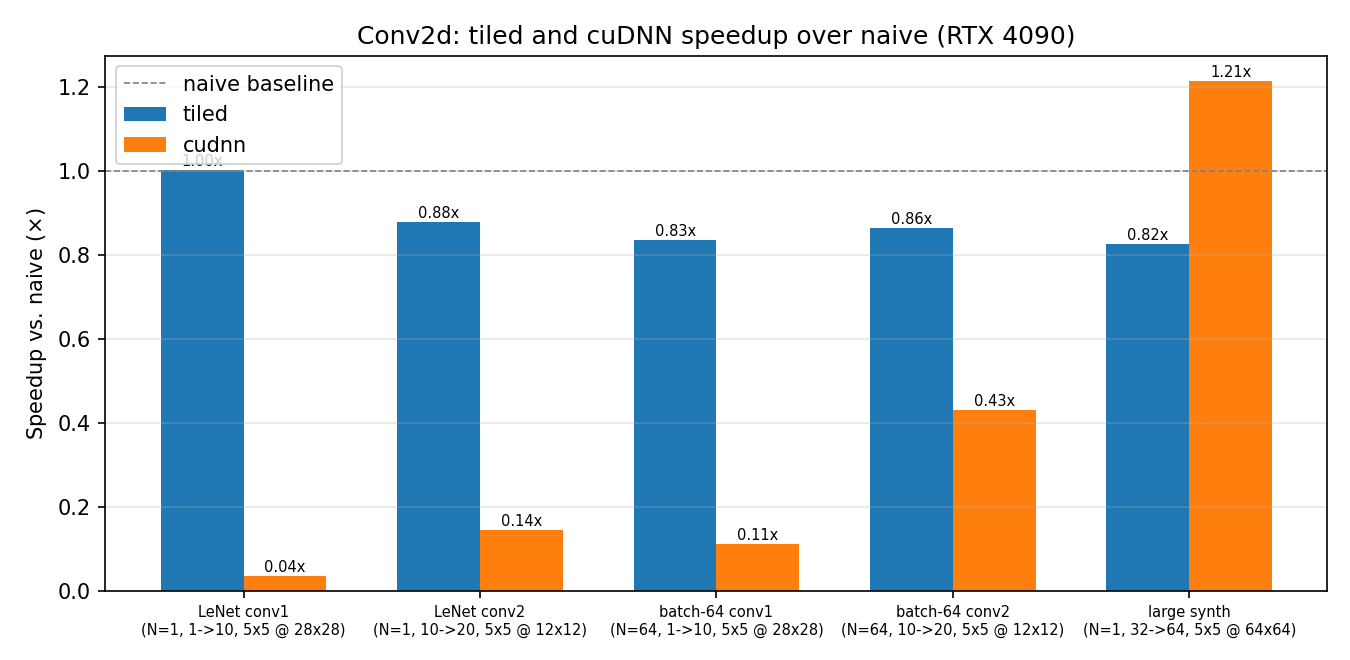
\includegraphics[width=\linewidth]{conv_bars.png}

    \vspace{0.2em}
    \scriptsize Per-shape bars, RTX 4090, 200 reps after warmup.
    \vfill
  \end{column}
  \end{columns}
\end{frame}

% ── Slide 5 ─ Tiled GEMM ─────────────────────────────────────────────────────
\begin{frame}{Tiled GEMM: where tiling actually wins}
  \begin{columns}[T,onlytextwidth]
  \begin{column}{0.48\textwidth}
    \vspace{1.4em}
    Same tiling idea applied to the fully-connected layers (matrix
    multiply $W\mathbf{x}$).

    \vspace{0.5em}
    Plot: fixed $1024{\times}1024$ problem, sweep batch size $N$.
    \begin{itemize}
      \item $N{=}1$: \textbf{3.8$\times$} (tile already reuses weights)
      \item $N{=}64$: \textbf{5.0$\times$}
      \item $N{=}256$: \textbf{6.1$\times$}
      \item $N{=}1024$: \textbf{6.4$\times$}
    \end{itemize}

    \vspace{0.3em}
    At LeNet's fc1 ($50{\times}320$) and fc2 ($10{\times}50$), the
    working set is tiny again --- tiled is only 1.06$\times$ / 1.01$\times$
    naive. Same \emph{regime} story: tiling pays when there's enough
    data to amortize the shmem load.
  \end{column}
  \begin{column}{0.52\textwidth}
    \vspace{1.4em}
    \centering
    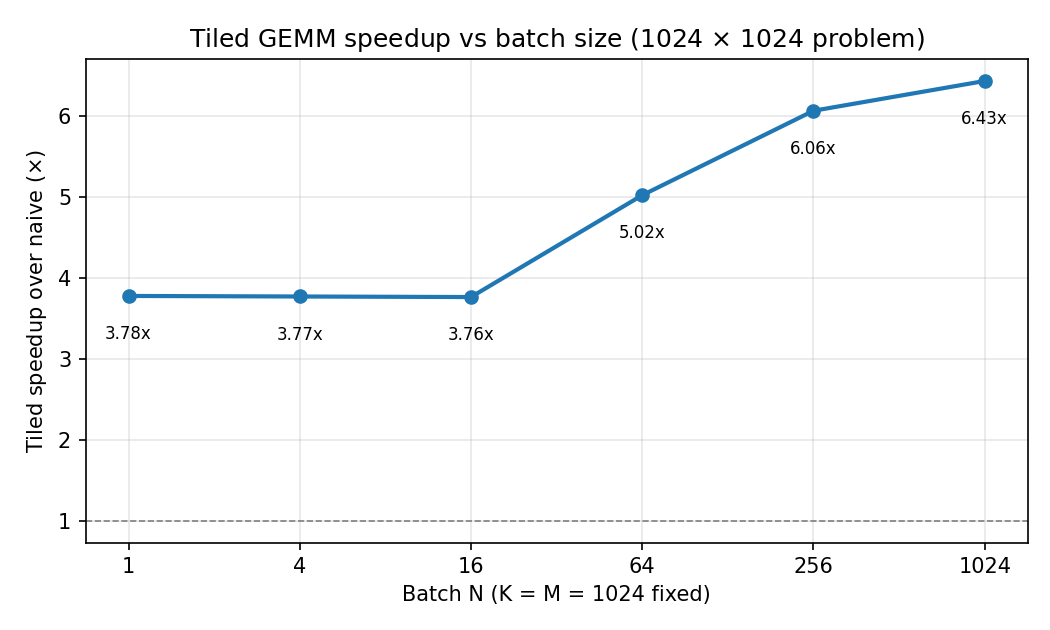
\includegraphics[width=\linewidth]{gemm_sweep.png}

    \vspace{0.3em}
    \scriptsize Tiled GEMM speedup vs batch size at $K{=}N{=}1024$.
  \end{column}
  \end{columns}
\end{frame}

% ── Slide 6 ─ Kernel Fusion ──────────────────────────────────────────────────
\begin{frame}{Opt.\ 3 --- conv + bias + ReLU + pool fused}
  \begin{columns}[T,onlytextwidth]
  \begin{column}{0.52\textwidth}
    \scriptsize Three back-to-back kernels at LeNet shapes spend more
    time on \textbf{launch overhead and DRAM round-trips} than arithmetic.
    \vspace{0.3em}
    \begin{center}
    \resizebox{0.97\linewidth}{!}{%
    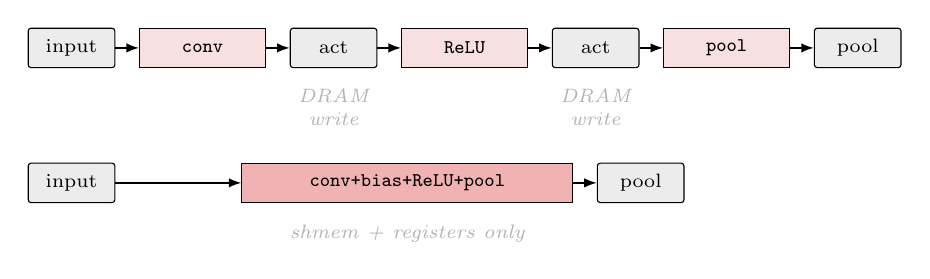
\begin{tikzpicture}[
      tnode/.style={draw, rectangle, rounded corners=1pt, minimum height=5mm,
                    minimum width=11mm, font=\scriptsize, inner sep=2pt,
                    fill=gray!15},
      kern/.style={draw, rectangle, minimum height=5mm, minimum width=16mm,
                   font=\scriptsize\tt, inner sep=2pt, fill=NURed!12},
      dram/.style={font=\scriptsize\itshape, text=gray!60},
      ar/.style={-{Latex[length=1.6mm,width=1.2mm]}, semithick},
      node distance=3mm,
    ]
      \node[tnode] (in1) {input};
      \node[kern, right=of in1] (c1) {conv};
      \node[tnode, right=of c1] (a1) {act};
      \node[kern, right=of a1] (r1) {ReLU};
      \node[tnode, right=of r1] (a2) {act};
      \node[kern, right=of a2] (p1) {pool};
      \node[tnode, right=of p1] (o1) {pool};
      \draw[ar] (in1)--(c1); \draw[ar] (c1)--(a1); \draw[ar] (a1)--(r1);
      \draw[ar] (r1)--(a2); \draw[ar] (a2)--(p1); \draw[ar] (p1)--(o1);
      \node[dram, below=1.5mm of a1, align=center] {DRAM\\write};
      \node[dram, below=1.5mm of a2, align=center] {DRAM\\write};
      \node[tnode, below=12mm of in1] (in2) {input};
      \node[kern, right=16mm of in2, minimum width=42mm, fill=NURed!30]
            (f) {conv+bias+ReLU+pool};
      \node[tnode, right=of f] (o2) {pool};
      \draw[ar] (in2)--(f); \draw[ar] (f)--(o2);
      \node[dram, below=1.5mm of f, align=center] {shmem + registers only};
    \end{tikzpicture}}
    \end{center}
    \vspace{0.2em}
    \scriptsize Each thread owns 4 conv accumulators in registers $\to$
    ReLU in place $\to$ 2$\times$2 max $\to$ one DRAM write.
  \end{column}
  \begin{column}{0.48\textwidth}
    \centering
    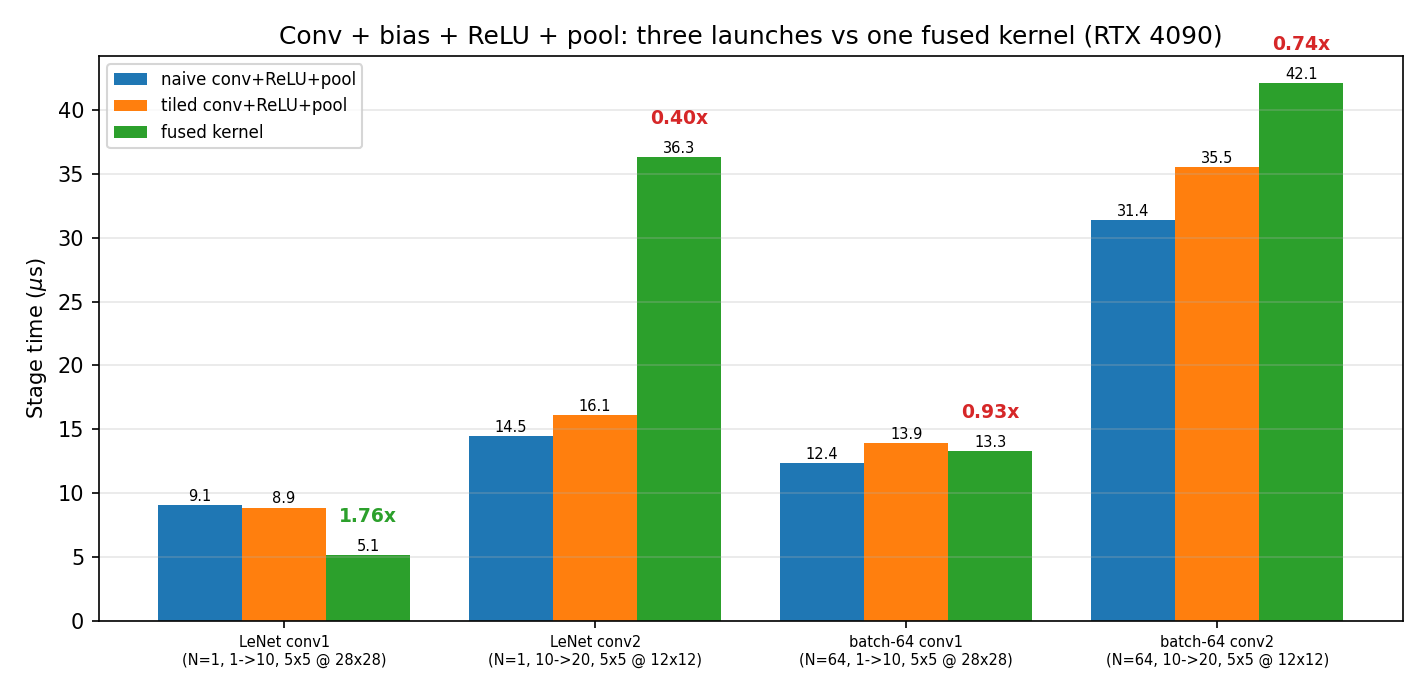
\includegraphics[width=\linewidth]{fused_bars.png}

    \vspace{0.3em}
    \scriptsize
    \textbf{conv1:} naive 1.76$\times$ slower (launch overhead bound). \\[0.2em]
    \textbf{conv2:} fused 0.40$\times$ naive --- only 320 threads on
    128 SMs, GPU starved. \\[0.2em]
    \textbf{Fusion is a latency trade, not a free win.}
  \end{column}
  \end{columns}
\end{frame}

% ── Slide 7 ─ Occupancy + cuDNN ──────────────────────────────────────────────
\begin{frame}{Resource usage and cuDNN reference}
  \begin{columns}[T,onlytextwidth]
  \begin{column}{0.57\textwidth}
    \scriptsize Static analysis via \texttt{nvcc -Xptxas=-v}
    (Nsight counters blocked on pod, unprivileged container).
    \vspace{0.2em}
    \begin{center}
    \begin{tabular}{@{}l c r r@{}}
      \toprule
      Kernel & Block & Regs & Smem \\
      \midrule
      \texttt{conv2d\_naive}           & 16$\times$16 & 39 & 0        \\
      \texttt{conv2d\_tiled}           & 16$\times$16 & 40 & 1600\,B  \\
      \texttt{conv\_relu\_pool\_fused} & 4$\times$4   & 39 & 576\,B   \\
      \texttt{linear\_naive}           & 256          & 38 & 0        \\
      \texttt{linear\_tiled}           & 16$\times$16 & 37 & 2048\,B  \\
      \texttt{max\_pool2d}             & 16$\times$16 & 20 & 0        \\
      \texttt{relu\_naive}             & 256          & 8  & 0        \\
      \texttt{log\_softmax}            & 16           & 15 & 64\,B    \\
      \bottomrule
    \end{tabular}
    \end{center}
    \scriptsize From \texttt{nvcc -Xptxas=-v}. No register spills.
    Naive-vs-tiled gap is a \textbf{memory-access-pattern} story, not
    resource usage. \texttt{log\_softmax} block=16 (half-warp) limits
    occupancy but costs only $\sim$1.8\,µs/call.
  \end{column}
  \begin{column}{0.43\textwidth}
    \centering
    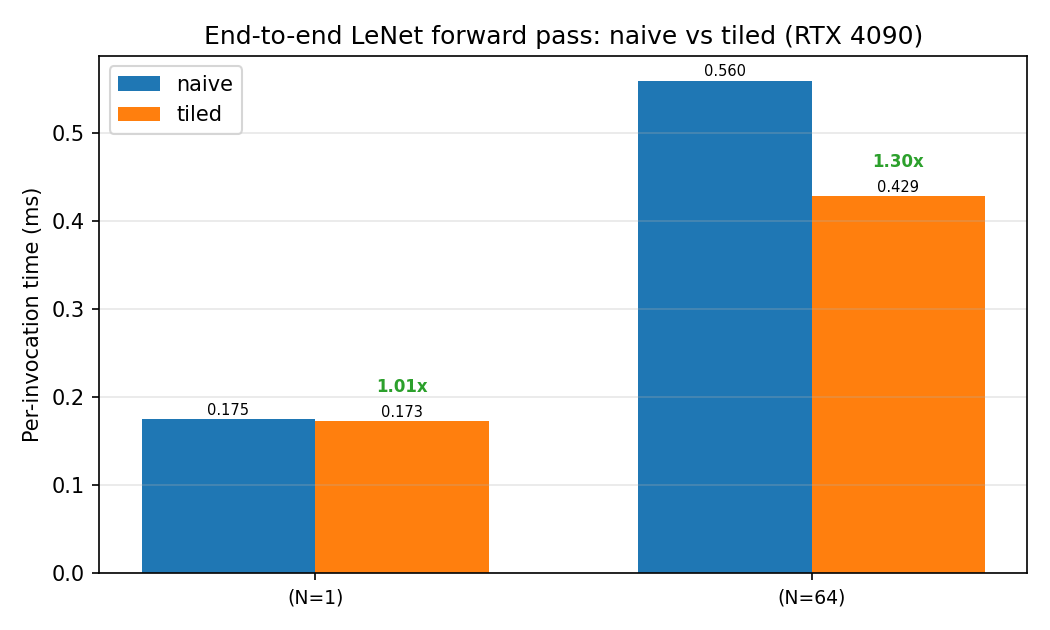
\includegraphics[width=\linewidth]{e2e_bars.png}

    \vspace{0.3em}
    \scriptsize Naive beats cuDNN at batch~1 (descriptor overhead).
    cuDNN defaults to TF32 on Ada: err $5.3\!\times\!10^{-3}$, 50$\times$
    our tolerance. Fixed by pinning \texttt{CUDNN\_FMA\_MATH}.
  \end{column}
  \end{columns}
\end{frame}

% ── Slide 8 ─ Demo ───────────────────────────────────────────────────────────
\begin{frame}[fragile]{Demo: it actually works}
  \begin{columns}[T,onlytextwidth]
  \begin{column}{0.52\textwidth}
    \textbf{Single-image inference} (RTX 4090):
    \begin{lstlisting}[language=bash,keywordstyle=\color{black},basicstyle=\ttfamily\scriptsize,xleftmargin=0pt,xrightmargin=10pt]
$ build/predict --bulk 42 --variant tiled
[predict] inference: 0.0312 ms
[predict] top-3 (log-prob):
  class 7 : -0.0001
  class 2 : -9.4823
  class 1 : -11.2144
[predict] argmax = 7  (label = 7)  OK
    \end{lstlisting}
  \end{column}
  \begin{column}{0.48\textwidth}
    \textbf{Correctness: 11\,/\,11 tests pass.}

    \vspace{0.4em}
    \scriptsize
    \begin{itemize}\setlength\itemsep{0.3em}
      \item CPU reference (hand-computed)
      \item \texttt{conv2d}: naive, tiled, cuDNN, fused
      \item \texttt{max\_pool2d}, \texttt{ReLU},
            \texttt{linear} (naive \& tiled),
            \texttt{log\_softmax}
      \item end-to-end forward pass
    \end{itemize}
  \end{column}
  \end{columns}

  \vspace{0.3em}
  \centering\footnotesize Plus the 10\,000-image MNIST parity harness:
  max abs err \textbf{1.91\,$\times$\,10$^{-5}$}, argmax-match on
  every image, accuracy 97.93\%.
\end{frame}

% ── Slide 9 ─ Discussion + Reflection ────────────────────────────────────────
\begin{frame}{Discussion and reflection}
  \begin{itemize}\setlength\itemsep{0.45em}
    \item \textbf{Tiling isn't default-on.} Same tile strategy hurts at
          LeNet, wins 6.4$\times$ on large GEMM. The regime decides.
    \item \textbf{Launch overhead is real.} Fusion buys 1.76$\times$ on
          \texttt{conv1}; starves SMs on \texttt{conv2}. Same kernel,
          opposite outcome depending on grid size.
    \item \textbf{FP32 $\neq$ cuDNN default.} TF32 on Ada breaks $10^{-4}$
          silently. Pin \texttt{CUDNN\_FMA\_MATH} explicitly.
    \item \textbf{Oracle chain paid off.} 11/11 per-kernel tests + 10k
          end-to-end parity --- no ``logits drifted'' debugging.
  \end{itemize}

  \vspace{0.5em}
  \begin{center}
  \textit{``The optimization'' and ``the speedup'' are separate things.}
  \end{center}

  \vspace{0.4em}
  \centering\normalsize\textbf{Thank you.}

  \smallskip
  \footnotesize\texttt{github.com/ashishdasu/cuda-cnn}
\end{frame}

\end{document}
